\begin{figure}[h]

\begin{center}
  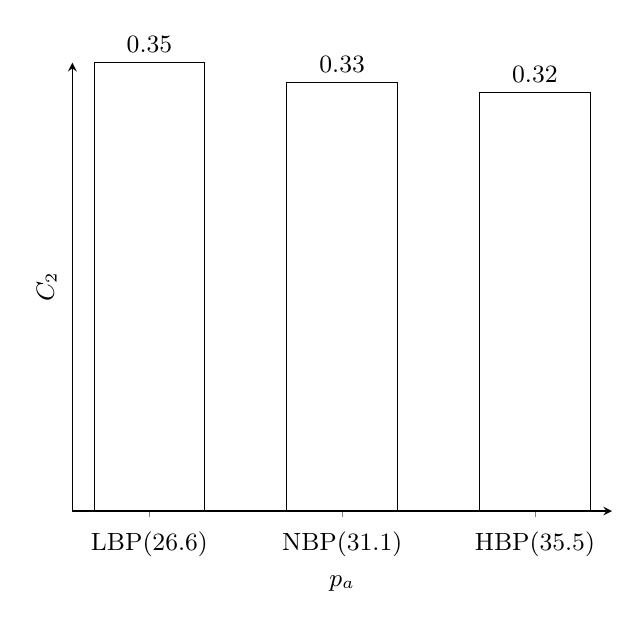
\begin{tikzpicture}[font=\small]
    \begin{axis}[
      ybar,
      bar width=40pt,
      xlabel={$p_a$},
      ylabel={$C_2$},
      ymin=0,
      ytick=\empty,
      xtick=data,
      axis x line=bottom,
      axis y line=left,
      enlarge x limits=0.2,
      %symbolic x coords={excellent,good,average,bad,awful},
      symbolic x coords = {LBP(26.6),NBP(31.1),HBP(35.5)},
      xticklabel style={anchor=base,yshift=-\baselineskip},
      nodes near coords={\pgfmathprintnumber\pgfplotspointmeta}
    ]
      \addplot[fill=white] coordinates {
        (LBP(26.6),0.345)
        (NBP(31.1),0.330)
        (HBP(35.5),0.322)
      };
    \end{axis}
  \end{tikzpicture}
  \end{center}
  \caption{$C_2 = f(p_a)$}
\end{figure}